\begin{figure}[H]
    \centering
    \scalebox{0.7}{%
    \begin{tikzpicture}[
      old/.style={draw=blue, fill=blue!15, circle, minimum size=7mm, inner sep=1pt, font=\small},
      pivot/.style={draw=red, fill=red!15, circle, minimum size=7mm, inner sep=1pt, font=\small},
      new/.style={draw=green!40!black, fill=green!15, circle, minimum size=7mm, inner sep=1pt, font=\small},
      every path/.style={thick},
      xscale=1.1, yscale=1.1,
      level distance=1.5cm, sibling distance=2cm,
      >=stealth,
    ]
    
    % --------------------------------------------------------------------
    % We draw exactly ONE depth-3 Geosodic Tree shape, color-coded:
    %  - The "old" depth-2 subtree on the left (blue)
    %  - The new pivot node at the top (red)
    %  - The new right subtree of depth-2 (green)
    %
    % Then we replicate that shape 3 times vertically,
    % just changing the *labels* on each copy.
    
    % Node counts total = 15 for depth-3:
    %  - Depth-2 subtree has 7 old nodes
    %  - 1 pivot node
    %  - Another depth-2 subtree has 7 new nodes
    
    %%%%%%%%%%%%%%%%%%%%%%%%%%%%%%%%%%%%%%%%%%%%%%%%
    % ============== FIRST ROW (1..15 in in-order) =
    %%%%%%%%%%%%%%%%%%%%%%%%%%%%%%%%%%%%%%%%%%%%%%%%
    \def\Yshift{0}
    
    % Left subtree (OLD, depth=2)
    \node[old] (OL)   at (-4, \Yshift - 1.0) {}; 
    \node[old] (OLL)  at (-6, \Yshift - 2.8) {};
    \node[old] (OLR)  at (-2, \Yshift - 2.8) {};
    \node[old] (OLLL) at (-7, \Yshift - 4.5) {};
    \node[old] (OLLR) at (-5, \Yshift - 4.5) {};
    \node[old] (OLRL) at (-3, \Yshift - 4.5) {};
    \node[old] (OLRR) at (-1, \Yshift - 4.5) {};
    
    % Pivot (RED)
    \node[pivot] (PIV) at (0, \Yshift + 0.5) {};
    
    % Right subtree (NEW, depth=2)
    \node[new] (NR)   at ( 4, \Yshift - 1.0) {}; 
    \node[new] (NRL)  at ( 2, \Yshift - 2.8) {}; % left child
    \node[new] (NRR)  at ( 6, \Yshift - 2.8) {}; % right child
    \node[new] (NRLL) at ( 1, \Yshift - 4.5) {};
    \node[new] (NRLR) at ( 3, \Yshift - 4.5) {};
    \node[new] (NRRL) at ( 5, \Yshift - 4.5) {};
    \node[new] (NRRR) at ( 7, \Yshift - 4.5) {};
    
    % Edges
    \draw (PIV) -- (OL);
    \draw (PIV) -- (NR);
    
    \draw (OL) -- (OLL);
    \draw (OL) -- (OLR);
    \draw (OLL) -- (OLLL);
    \draw (OLL) -- (OLLR);
    \draw (OLR) -- (OLRL);
    \draw (OLR) -- (OLRR);
    
    \draw (NR) -- (NRL);
    \draw (NR) -- (NRR);
    \draw (NRL) -- (NRLL);
    \draw (NRL) -- (NRLR);
    \draw (NRR) -- (NRRL);
    \draw (NRR) -- (NRRR);
    
    % In-order labeling: 
    % Left subtree: OLLL->1, OLL->2, OLLR->3, OL->4, OLRL->5, OLR->6, OLRR->7
    % Pivot -> 8
    % Right subtree: NRLL->9, NRL->10, NRLR->11, NR->12, NRRL->13, NRR->14, NRRR->15
    \node[old]   at (OLLL) {1};
    \node[old]   at (OLL)  {2};
    \node[old]   at (OLLR) {3};
    \node[old]   at (OL)   {4};
    \node[old]   at (OLRL) {5};
    \node[old]   at (OLR)  {6};
    \node[old]   at (OLRR) {7};
    
    \node[pivot] at (PIV)  {8};
    
    \node[new]   at (NRLL) {9};
    \node[new]   at (NRL)  {10};
    \node[new]   at (NRLR) {11};
    \node[new]   at (NR)   {12};
    \node[new]   at (NRRL) {13};
    \node[new]   at (NRR)  {14};
    \node[new]   at (NRRR) {15};
    
    \node[draw=none,fill=none,font=\bfseries]
          at (0, \Yshift + 1.6)
          {Depth-3 Geosodic Tree --- In-order $\{1,\dots,15\}$};
    
    
    %%%%%%%%%%%%%%%%%%%%%%%%%%%%%%%%%%%%%%%%%%%%%%%%%%%%%%%%%%%%%%%%%%%%
    % ===== SECOND ROW (fractions n/2^{n-1} or n/16 for d=3) ===========
    %%%%%%%%%%%%%%%%%%%%%%%%%%%%%%%%%%%%%%%%%%%%%%%%%%%%%%%%%%%%%%%%%%%%
    \def\Yshift{-8}
    
    % Repeat the same shape (old/pivot/new) with a Y offset:
    \node[old] (OL2)   at (-4, \Yshift - 1.0) {};
    \node[old] (OLL2)  at (-6, \Yshift - 2.8) {};
    \node[old] (OLR2)  at (-2, \Yshift - 2.8) {};
    \node[old] (OLLL2) at (-7, \Yshift - 4.5) {};
    \node[old] (OLLR2) at (-5, \Yshift - 4.5) {};
    \node[old] (OLRL2) at (-3, \Yshift - 4.5) {};
    \node[old] (OLRR2) at (-1, \Yshift - 4.5) {};
    
    \node[pivot] (PIV2) at (0, \Yshift + 0.5) {};
    
    \node[new] (NR2)   at ( 4, \Yshift - 1.0) {};
    \node[new] (NRL2)  at ( 2, \Yshift - 2.8) {};
    \node[new] (NRR2)  at ( 6, \Yshift - 2.8) {};
    \node[new] (NRLL2) at ( 1, \Yshift - 4.5) {};
    \node[new] (NRLR2) at ( 3, \Yshift - 4.5) {};
    \node[new] (NRRL2) at ( 5, \Yshift - 4.5) {};
    \node[new] (NRRR2) at ( 7, \Yshift - 4.5) {};
    
    % Edges
    \draw (PIV2) -- (OL2);
    \draw (PIV2) -- (NR2);
    
    \draw (OL2) -- (OLL2);
    \draw (OL2) -- (OLR2);
    \draw (OLL2) -- (OLLL2);
    \draw (OLL2) -- (OLLR2);
    \draw (OLR2) -- (OLRL2);
    \draw (OLR2) -- (OLRR2);
    
    \draw (NR2) -- (NRL2);
    \draw (NR2) -- (NRR2);
    \draw (NRL2) -- (NRLL2);
    \draw (NRL2) -- (NRLR2);
    \draw (NRR2) -- (NRRL2);
    \draw (NRR2) -- (NRRR2);
    
    % In-order fractional labels: ( n/16 for n=1..15 )
    \node[old]   at (OLLL2) {$\tfrac{1}{16}$};
    \node[old]   at (OLL2)  {$\tfrac{2}{16}$};
    \node[old]   at (OLLR2) {$\tfrac{3}{16}$};
    \node[old]   at (OL2)   {$\tfrac{4}{16}$};
    \node[old]   at (OLRL2) {$\tfrac{5}{16}$};
    \node[old]   at (OLR2)  {$\tfrac{6}{16}$};
    \node[old]   at (OLRR2) {$\tfrac{7}{16}$};
    
    \node[pivot] at (PIV2) {$\tfrac{8}{16}$};
    
    \node[new]   at (NRLL2) {$\tfrac{9}{16}$};
    \node[new]   at (NRL2)  {$\tfrac{10}{16}$};
    \node[new]   at (NRLR2) {$\tfrac{11}{16}$};
    \node[new]   at (NR2)   {$\tfrac{12}{16}$};
    \node[new]   at (NRRL2) {$\tfrac{13}{16}$};
    \node[new]   at (NRR2)  {$\tfrac{14}{16}$};
    \node[new]   at (NRRR2) {$\tfrac{15}{16}$};
    
    \node[draw=none,fill=none,font=\bfseries]
          at (0, \Yshift + 1.6)
          {Depth-3 --- Labels $n/2^{d+1}$ (viewing $d=3$)};
    
    
    %%%%%%%%%%%%%%%%%%%%%%%%%%%%%%%%%%%%%%%%%%%%%%%%%%%%%%%%%%%%%%%%%%%%
    % =========== THIRD ROW (4-bit binary 0001..1111) ==================
    %%%%%%%%%%%%%%%%%%%%%%%%%%%%%%%%%%%%%%%%%%%%%%%%%%%%%%%%%%%%%%%%%%%%
    \def\Yshift{-16}
    
    \node[old] (OL3)   at (-4, \Yshift - 1.0) {};
    \node[old] (OLL3)  at (-6, \Yshift - 2.8) {};
    \node[old] (OLR3)  at (-2, \Yshift - 2.8) {};
    \node[old] (OLLL3) at (-7, \Yshift - 4.5) {};
    \node[old] (OLLR3) at (-5, \Yshift - 4.5) {};
    \node[old] (OLRL3) at (-3, \Yshift - 4.5) {};
    \node[old] (OLRR3) at (-1, \Yshift - 4.5) {};
    
    \node[pivot] (PIV3) at (0, \Yshift + 0.5) {};
    
    \node[new] (NR3)   at ( 4, \Yshift - 1.0) {};
    \node[new] (NRL3)  at ( 2, \Yshift - 2.8) {};
    \node[new] (NRR3)  at ( 6, \Yshift - 2.8) {};
    \node[new] (NRLL3) at ( 1, \Yshift - 4.5) {};
    \node[new] (NRLR3) at ( 3, \Yshift - 4.5) {};
    \node[new] (NRRL3) at ( 5, \Yshift - 4.5) {};
    \node[new] (NRRR3) at ( 7, \Yshift - 4.5) {};
    
    % Edges
    \draw (PIV3) -- (OL3);
    \draw (PIV3) -- (NR3);
    
    \draw (OL3) -- (OLL3);
    \draw (OL3) -- (OLR3);
    \draw (OLL3) -- (OLLR3);
    \draw (OLL3) -- (OLLL3);
    \draw (OLR3) -- (OLRL3);
    \draw (OLR3) -- (OLRR3);
    
    \draw (NR3) -- (NRL3);
    \draw (NR3) -- (NRR3);
    \draw (NRL3) -- (NRLL3);
    \draw (NRL3) -- (NRLR3);
    \draw (NRR3) -- (NRRL3);
    \draw (NRR3) -- (NRRR3);
    
    % In-order binary: from 0001..1111
    \node[old]   at (OLLL3) {0001};
    \node[old]   at (OLL3)  {0010};
    \node[old]   at (OLLR3) {0011};
    \node[old]   at (OL3)   {0100};
    \node[old]   at (OLRL3) {0101};
    \node[old]   at (OLR3)  {0110};
    \node[old]   at (OLRR3) {0111};
    
    \node[pivot] at (PIV3) {1000};
    
    \node[new]   at (NRLL3) {1001};
    \node[new]   at (NRL3)  {1010};
    \node[new]   at (NRLR3) {1011};
    \node[new]   at (NR3)   {1100};
    \node[new]   at (NRRL3) {1101};
    \node[new]   at (NRR3)  {1110};
    \node[new]   at (NRRR3) {1111};
    
    \node[draw=none,fill=none,font=\bfseries]
          at (0, \Yshift + 1.6)
          {Depth-3 --- Binary labels `0001`--`1111`};
    
    \end{tikzpicture}
    } % end scalebox
    \caption{A single Geosodic Tree at depth 3 (15 nodes) with three different 
    “auxiliary” labelings. Top: natural numbers 1--15 in proper in-order. 
    Middle: fractional labels \(\tfrac{n}{16}\) for \(n=1\ldots15\) -- at each pivot, we decide whether to add or subtract 
    \(\tfrac{1}{16}\) according to left or right and create a partial sum that approximates any real [0,1] to an arbitrary precision depth d. 
    Bottom: 4-bit binary from `0001` to `1111`. 
    In each drawing, the \textcolor{blue}{old depth-2 nodes} remain, the 
    \textcolor{red}{pivot node} is newly placed, and the 
    \textcolor{green!30!black}{new} depth-2 subtree is attached on the right, 
    illustrating meltdown-free expansion from depth 2 to depth 3.}
    \label{fig:depth3-alt-labels}
    \end{figure}
    